\documentclass[a4paper,twoside,11pt]{article}
\usepackage[utf8]{inputenc}
\usepackage[english]{babel}
\usepackage{graphicx}
\usepackage{url}
\usepackage{float}

% pdflatex

% redefinição das margens das páginas
\setlength{\textheight}{24.00cm}
\setlength{\textwidth}{15.50cm}
\setlength{\topmargin}{0.35cm}
\setlength{\headheight}{0cm}
\setlength{\headsep}{0cm}
\setlength{\oddsidemargin}{0.25cm}
\setlength{\evensidemargin}{0.25cm}
\setlength{\textfloatsep}{16pt}

\begin{document}

\begin{figure}[t]
\centering

\includegraphics [width=5in]{logoISEL.png}
\end{figure}

\title{\huge \textbf{WaveCoach}\\[1ex]\LARGE Training Management Platform for Surf}

\author{
\begin{tabular}{c}
             Tiago Canilhas, n.º50472, e-mail: a50472@alunos.isel.pt, tel.: 924115540\\
             João Barrisco, n.º50476, e-mail: a50476@alunos.isel.pt, tel.: 967487235\\
\end{tabular}}

\date{
\begin{tabular}{ll}
  {Supervisor:} Filipe Freitas, e-mail: ffreitas@cc.isel.ipl.pt \\
\end{tabular}\\
\vspace{5mm}
April 28,  2025}

\maketitle

\section{Introduction}
The goal of this project is to develop a web application that allows the management of surfing athletes. This application is mainly aimed at coaches, but athletes can also access it to view their performance. Coaches will be able to register athletes, log different training sessions (e.g. gym, surf), record competition results, and monitor
performance through interactive charts. This will help them analyze progress and adjust training plans. This project is being developed to meet coaches' need for a more efficient and effective platform, replacing manual registration, which can be time-consuming and difficult to manage as the number of athletes grows. The platform not only saves time but also ensures greater accuracy and accessibility of data, allowing coaches to focus more on their athletes’ development and less on administrative tasks.

\section{Accomplished Tasks}


\subsection{Backend}

\subsubsection{Technologies}
\begin{itemize}
\item Kotlin
\item Spring Framework
\item Java Database Interface (JDBI)
\item PostgresSQL
\end{itemize}

\subsubsection{Entitity Relationship Model}

\begin{figure}[H]
\centering
\includegraphics[width=6in]{EA.png}
\caption{Entity Relationship Model}
\end{figure}

\subsubsection{Backend Organization}
\begin{figure}[H]
\centering
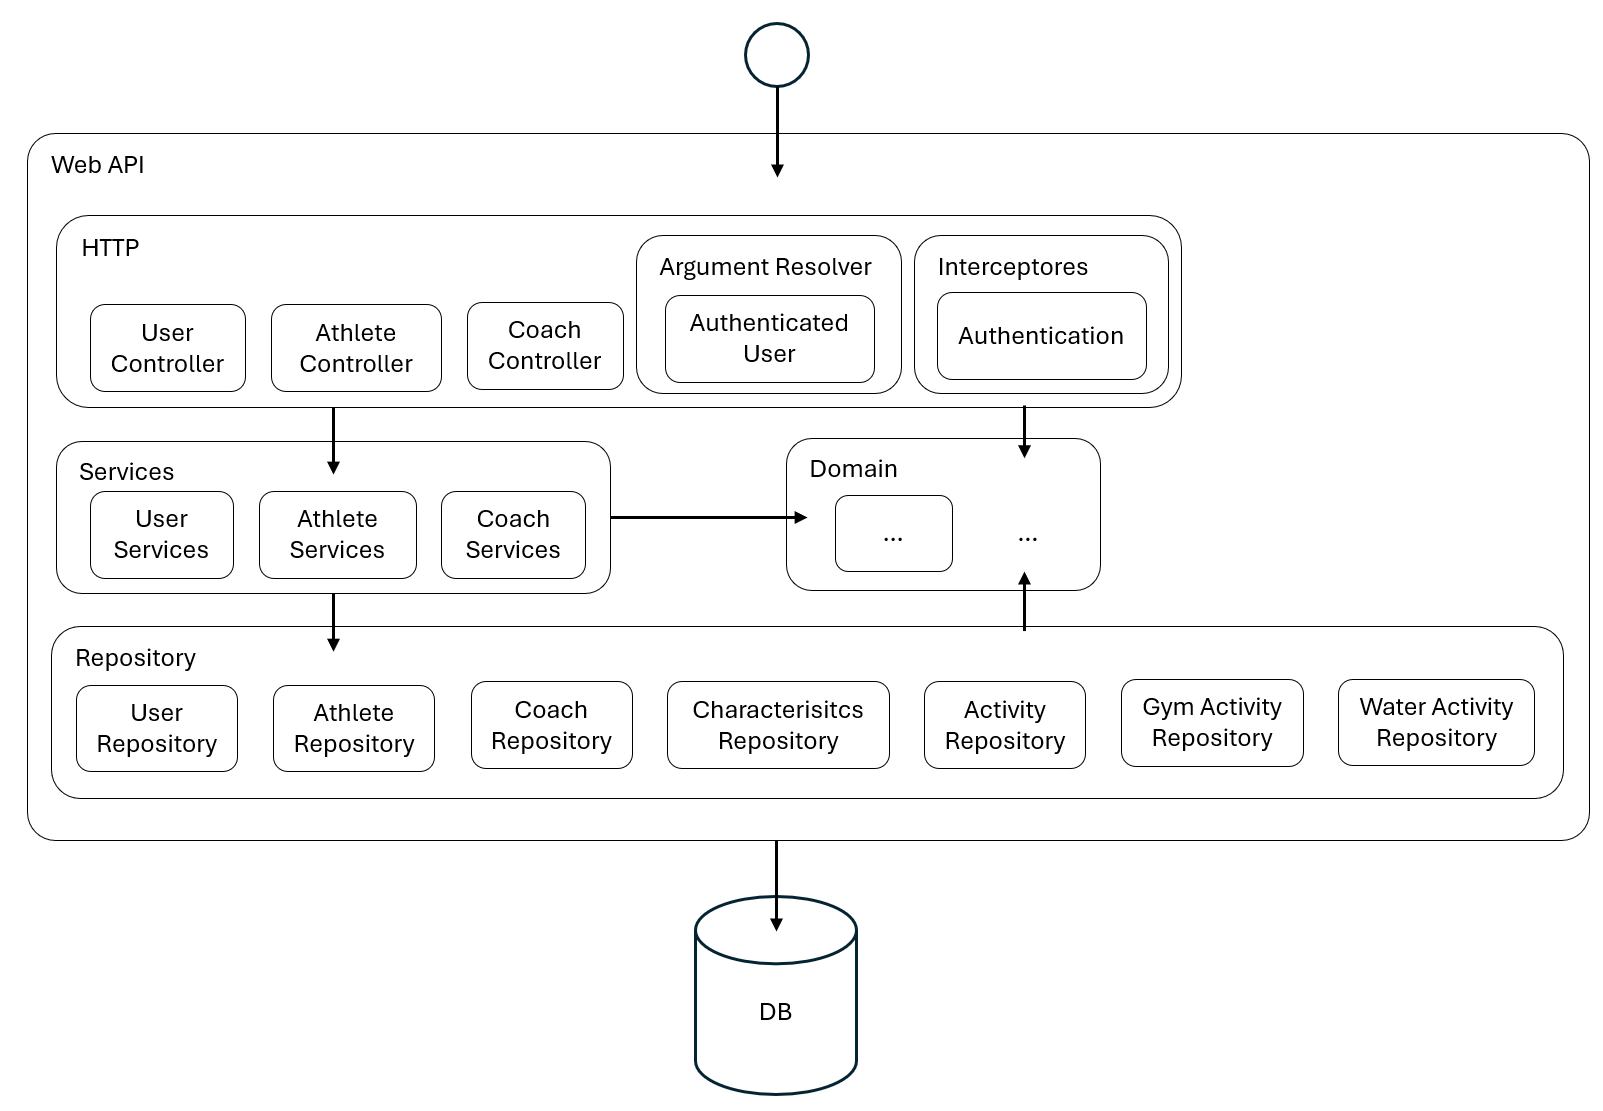
\includegraphics[width=5in]{BackendDiagram.png}
\caption{Backend Diagram}
\end{figure}

\subsubsection{User Registration}
\subsubsection{Athlete management}
\subsubsection{Athlete Profile}

\subsection{Frontend}

\subsubsection{Technologies}
\begin{itemize}
\item Typescript
\item React
\item CSS Module
\item Webpack
\end{itemize}

\subsubsection{Frontend Organization}

\begin{figure}[H]
\centering
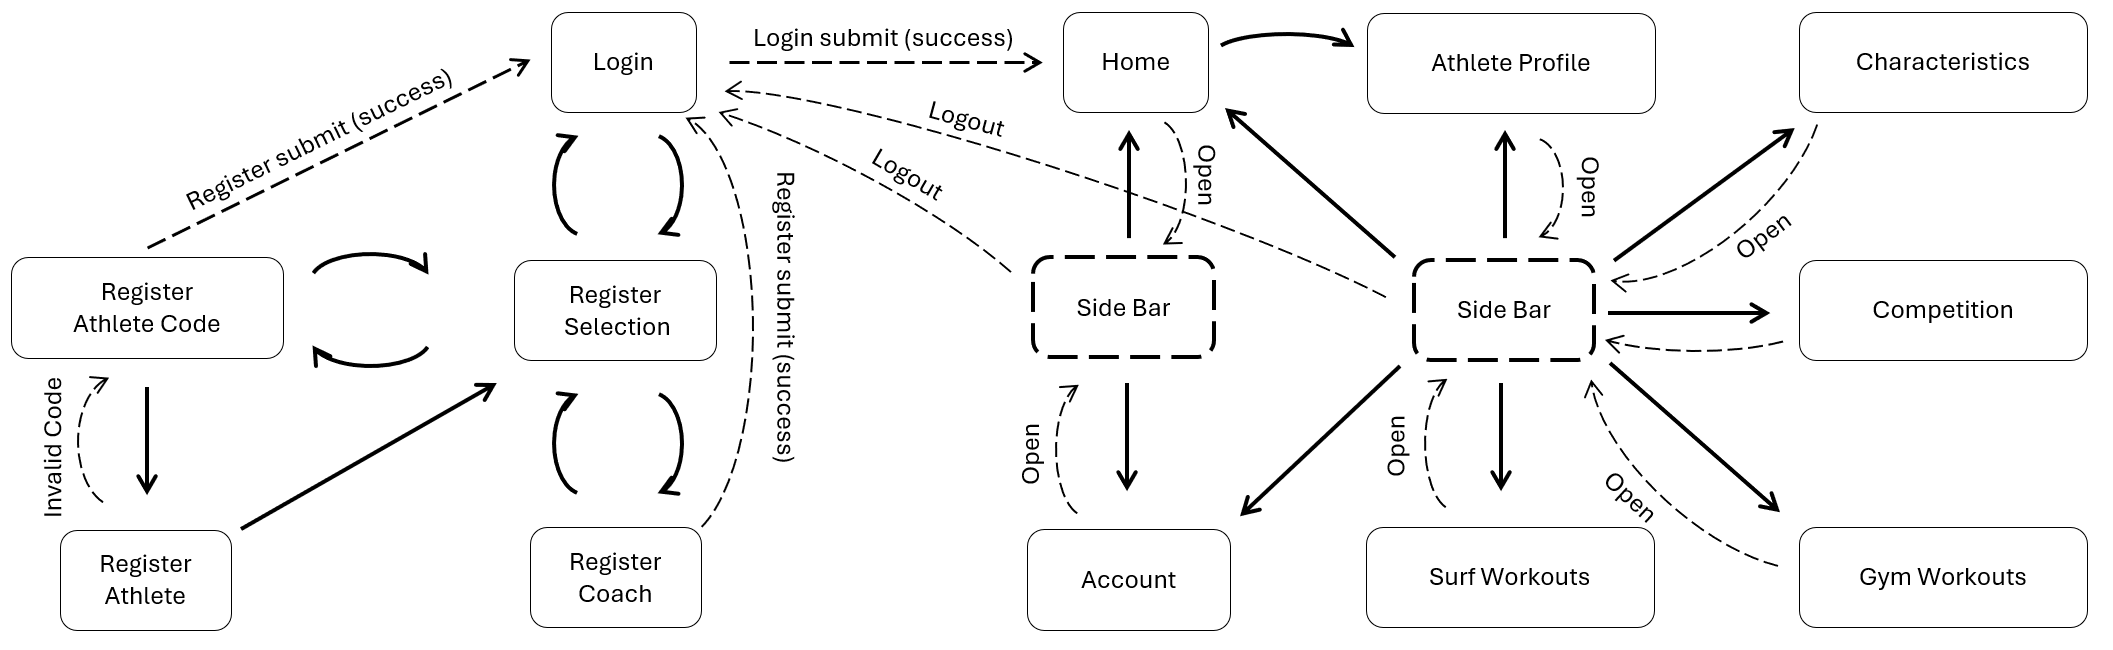
\includegraphics[width=5in]{ViewsDiagram.png}
\caption{Views Diagram}
\end{figure}

\subsubsection{User Registration}
\subsubsection{Athlete management}
\subsubsection{Athlete Profile}


\section{Pending Tasks}
\subsection{Athletes' training records}
\subsection{Athletes' summaries}
\subsection{Athletes' competition records}
\subsection{Mobile App (new)}

% \bibliographystyle{unsrt}
% \bibliography{references}

\end{document}